% ===================================================================
% 4. Experiments
% ===================================================================
\section{Experiments}
\label{sec:exp}

% ------------------------------------------------------------------
\subsection{Experimental Protocol}
\label{sec:exp_protocol}

\paragraph{Dataset and split}
We evaluate on LineMod~\cite{hinterstoisser2012model} (13 objects, RGB-D, cluttered scenes) under the \emph{official} per-object split shipped with the dataset --- the same protocol as DenseFusion~\cite{wang2019densefusion}. About 15\% of the frames of each sequence are used for training and the remaining 85\% for testing: 2{,}373 training and 13{,}407 test images overall. A validation set (357 images) is carved out of the training pool for model selection and early stopping. The test set is never used for any training or selection decision, and we use \textbf{no synthetic or rendered training images}: all learning happens on the 2{,}016 real frames. Split integrity (disjointness and per-object counts) is asserted programmatically at data-loading time.

\paragraph{Metric}
We report the standard ADD accuracy: a pose is correct if the average distance between model points transformed by the predicted and ground-truth poses is below 10\% of the object diameter. For the two symmetric objects (eggbox, glue) we use the closest-point variant ADD-S. Diameters are taken from the dataset's \texttt{models\_info} file; $N{=}500$ model points are used throughout.

\paragraph{Training}
All pose models are trained with Adam (lr $10^{-4}$, weight decay $10^{-4}$), batch size 64, ADD loss (Eq.~\ref{eq:add_loss}), \texttt{ReduceLROnPlateau} scheduling, and early stopping on validation ADD (patience 30, epoch cap 400). Photometric augmentation only (Sec.~\ref{sec:method_fusion}).

% ------------------------------------------------------------------
\subsection{Phase 2: Object Detection}
\label{sec:exp_detection}

YOLO11n is fine-tuned for 100 epochs on the official training frames only. On the 13{,}407 test images it reaches 99.5 mAP@50 and 94.2 mAP@50-95, with 99.98 precision and 99.99 recall, and produces a usable box for every frame (zero detection misses at confidence 0.25): the downstream pose evaluation can therefore be fully end-to-end. Detection on LineMod remains reliable even in the low-data regime; this matters for our pipeline because the box is also used to compute the geometric anchor (Sec.~\ref{sec:method_anchor}).

% ------------------------------------------------------------------
\subsection{Phase 3: RGB-only Baseline}
\label{sec:exp_rgb_baseline}

Table~\ref{tab:phase3} disentangles rotation and translation for the RGB-only baseline by swapping the translation source while keeping the predicted rotation fixed. Rotation is learnable from RGB crops: with an oracle translation the baseline reaches 76.7\% ADD(-S), and the score is identical whether the crop comes from ground-truth or predicted boxes --- further evidence that detection is not a bottleneck. Translation is not: the pinhole approximation collapses to 7.5\% (its spherical-object assumption fails on elongated geometries), and direct regression from RGB features to 1.1\%. Phase~4 addresses this failure mode.

\begin{table}[t]
    \centering
    \caption{Phase-3 (RGB-only) on the official test set: predicted rotation combined with different translation sources. ADD(-S), \%.}
    \label{tab:phase3}
    \small
    \begin{tabular}{@{}lc@{}}
        \toprule
        \textbf{Configuration} & \textbf{ADD(-S) \%} \\
        \midrule
        GT crop + oracle translation & 76.7 \\
        YOLO crop + oracle translation & 76.7 \\
        YOLO crop + pinhole translation & 7.5 \\
        YOLO crop + regressed translation & 1.1 \\
        \bottomrule
    \end{tabular}
\end{table}

% ------------------------------------------------------------------
\subsection{Phase 4: Ablation of the Translation Formulation}
\label{sec:exp_ablation}

Table~\ref{tab:ablation} isolates the contribution of the anchored residual formulation (Sec.~\ref{sec:method_anchor}) by keeping the architecture ($\sim$36M parameters), the training data, and the recipe fixed, and varying only the geometry input and the regression target. Two learning-free references bound the table: copying the per-object \emph{mean training pose} scores 0.4\%, and combining the anchor with the mean training rotation scores 10.4\% --- the score obtainable from the geometric prior alone, with zero learning.

\begin{table}[t]
    \centering
    \caption{Ablation on the official LineMod test set (13{,}407 images, ground-truth boxes). Same architecture, data, and recipe; only the geometry input and the translation target change. $^\dagger$learning-free references.}
    \label{tab:ablation}
    \small
    \begin{tabular}{@{}lccc@{}}
        \toprule
        \textbf{Variant} & \textbf{Anchor} & \textbf{ADD(-S) \%} & \textbf{Err.\ (mm)} \\
        \midrule
        Mean train pose$^\dagger$      & --     & 0.4  & --   \\
        Anchor + mean rotation$^\dagger$ & \checkmark & 10.4 & 58.0 \\
        \midrule
        \texttt{raw} (absolute regr.)  & --     & 6.8  & 69.7 \\
        \texttt{norm}                  & \checkmark & \textbf{95.2} & \textbf{9.1} \\
        \texttt{xyz}                   & \checkmark & 94.8 & 10.1 \\
        \bottomrule
    \end{tabular}
\end{table}

\begin{figure}[t]
    \centering
    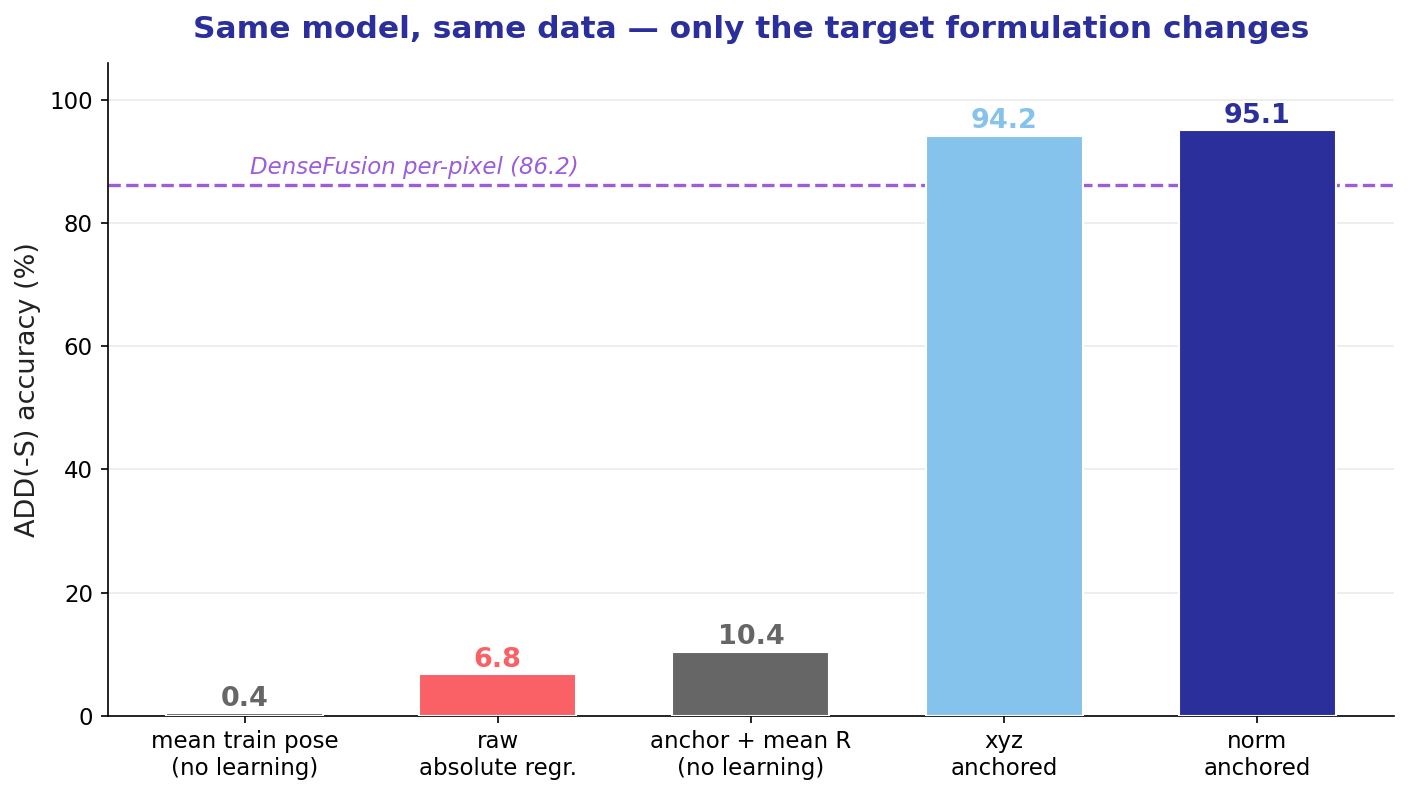
\includegraphics[width=\columnwidth]{figure/v2/ablation_bars.png}
    \caption{Visual summary of Table~\ref{tab:ablation}: with model, data, and recipe fixed, anchoring the translation target moves the same network from below the learning-free reference to above the DenseFusion per-pixel baseline.}
    \label{fig:ablationbars}
\end{figure}

Three observations. First, direct absolute regression (6.8\%) performs \emph{below} the learning-free anchor reference (10.4\%): the network cannot even recover the information that the depth median already provides, confirming that the failure is in the formulation of the target rather than in the amount of data. Second, anchoring the target transforms the same model into an accurate estimator (95.2\%), with the mean error dropping from 69.7 to 9.1\,mm. Third, the anchored normalized depth and the anchored XYZ map perform equivalently: once the \emph{target} is expressed relative to observed geometry, enriching the \emph{input} encoding adds little. Across three independent training seeds, the \texttt{norm} variant scores $94.9 \pm 0.2$\%, indicating that the result is not seed-dependent.

% ------------------------------------------------------------------
\subsection{End-to-End Evaluation}
\label{sec:exp_results}

Table~\ref{tab:perclass} reports the per-class end-to-end results: the YOLO11n boxes are used for the crop, the metadata vector, \emph{and} the anchor, and any detection miss would count as a pose failure. The degradation with respect to ground-truth boxes is negligible ($95.2 \rightarrow 95.1$ for \texttt{norm}): the median-based anchor is robust to the localization jitter of the real detector.

\begin{table}[t]
    \centering
    \caption{Per-class end-to-end ADD(-S) accuracy (\%) on the official LineMod test set, with predicted detections used for crop, metadata, and anchor. $^*$symmetric objects, evaluated with ADD-S.}
    \label{tab:perclass}
    \small
    \begin{tabular}{@{}lcc@{}}
        \toprule
        \textbf{Object} & \texttt{norm} & \texttt{xyz} \\
        \midrule
        ape          & 89.8 & 86.6 \\
        benchvise    & 96.6 & 95.6 \\
        camera       & 94.3 & 95.4 \\
        can          & 95.9 & 94.3 \\
        cat          & 98.1 & 96.7 \\
        driller      & 94.3 & 92.8 \\
        duck         & 87.6 & 84.9 \\
        eggbox$^*$   & 100.0 & 99.9 \\
        glue$^*$     & 99.3 & 99.6 \\
        holepuncher  & 93.2 & 91.8 \\
        iron         & 95.1 & 95.2 \\
        lamp         & 97.9 & 97.0 \\
        phone        & 94.2 & 94.1 \\
        \midrule
        \textbf{Mean} & \textbf{95.1} & 94.2 \\
        \bottomrule
    \end{tabular}
\end{table}

\begin{figure}[t]
    \centering
    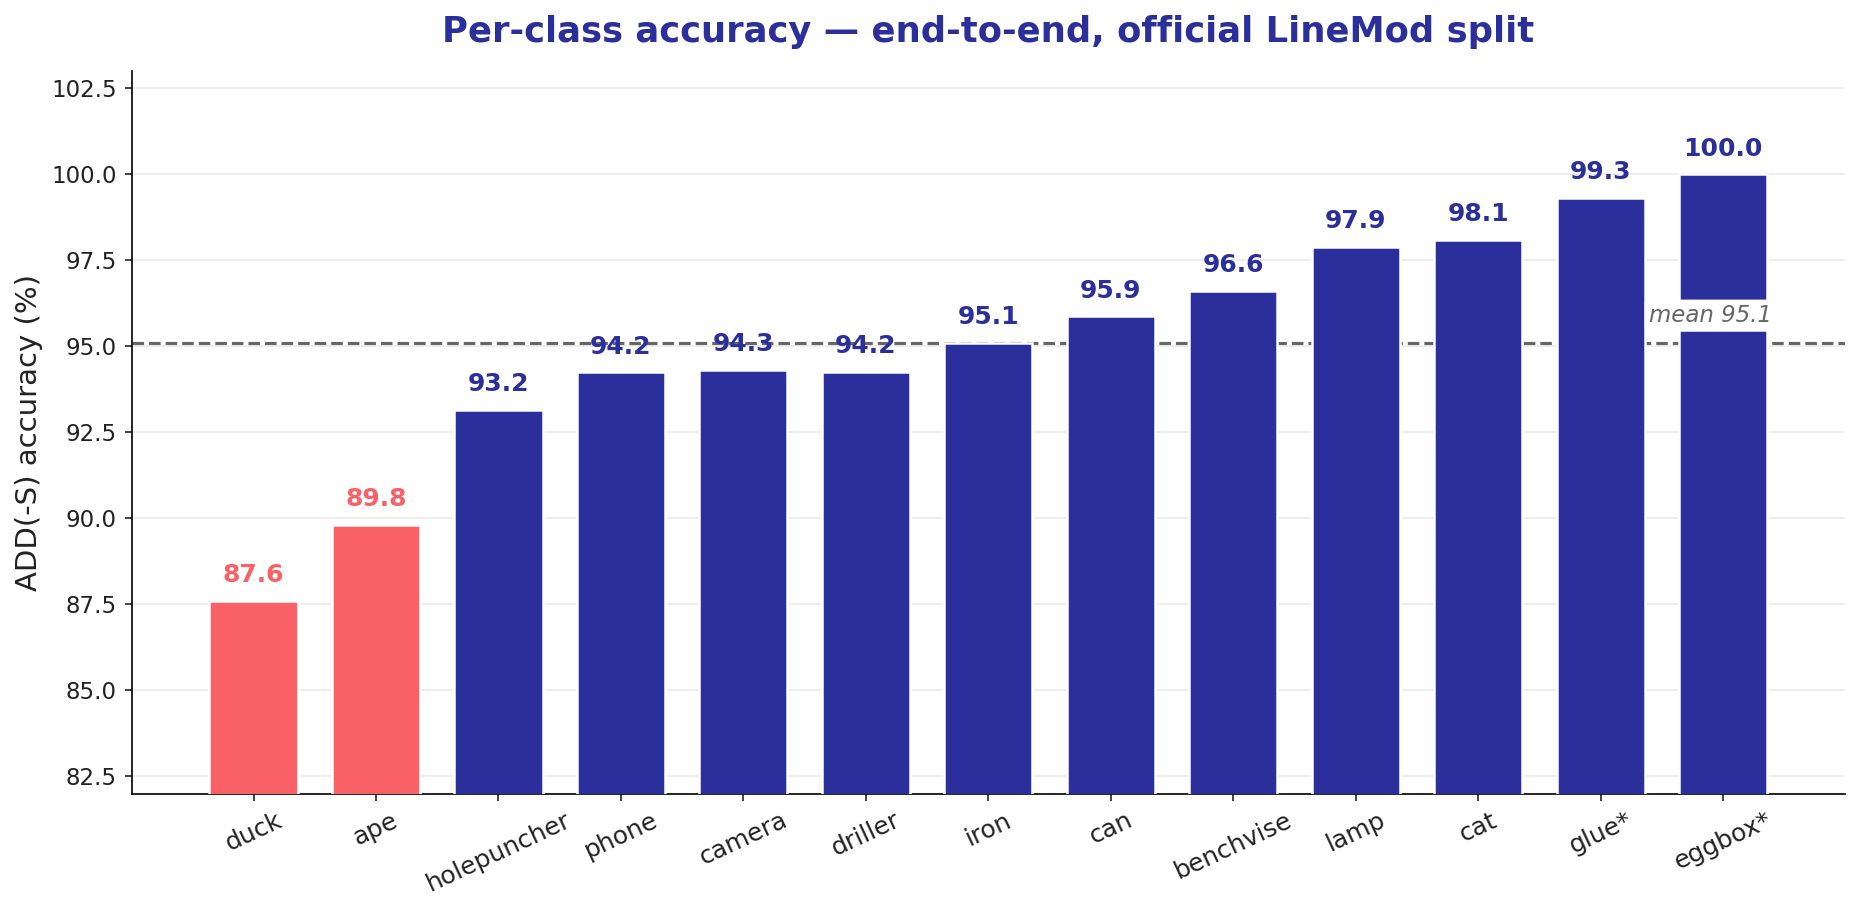
\includegraphics[width=\columnwidth]{figure/v2/perclass_e2e.png}
    \caption{Per-class end-to-end accuracy of the \texttt{norm} variant. The two classes below 90\% are the two physically smallest objects.}
    \label{fig:perclassbar}
\end{figure}

The two weakest classes (duck 87.6\%, ape 89.8\%) are the two physically smallest objects: with diameters of 109 and 102\,mm, their ADD acceptance thresholds are 10--11\,mm, so the same absolute error that passes on larger objects fails on them. This is a property of the relative threshold rather than a per-class failure mode: their mean errors (7--8\,mm) are in line with the rest of the dataset.

\paragraph{Comparison with the state of the art}
Table~\ref{tab:sota} positions our result under the official protocol. Among methods trained on \emph{real images only}, our anchored global fusion obtains the highest accuracy, above the per-pixel variant of DenseFusion and comparable to its iteratively refined variant, without dense per-point fusion or a refinement stage. Keypoint-voting methods trained with large amounts of additional synthetic images per object~\cite{he2020pvn3d, he2021ffb6d} remain about 4.5 points ahead.

\begin{table}[t]
    \centering
    \caption{ADD(-S) accuracy on LineMod under the official protocol. ``+synth'' methods add rendered synthetic training images; baseline numbers are taken from the respective original papers.}
    \label{tab:sota}
    \small
    \begin{tabular}{@{}lccc@{}}
        \toprule
        \textbf{Method} & \textbf{Data} & \textbf{Refine} & \textbf{ADD(-S) \%} \\
        \midrule
        DenseFusion (per-pixel)~\cite{wang2019densefusion} & real & -- & 86.2 \\
        DenseFusion (iterative)~\cite{wang2019densefusion} & real & \checkmark & 94.3 \\
        \textbf{Ours (\texttt{norm}, end-to-end)} & real & -- & \textbf{95.1} \\
        \midrule
        PVN3D~\cite{he2020pvn3d} & real+synth & -- & 99.4 \\
        FFB6D~\cite{he2021ffb6d} & real+synth & -- & 99.7 \\
        \bottomrule
    \end{tabular}
\end{table}

% ------------------------------------------------------------------
\subsection{Memorization Analysis}
\label{sec:exp_memorization}

Because LineMod sequences are densely sampled videos, a high accuracy could in principle reflect retrieval of similar training views rather than genuine pose estimation. We quantify this hypothesis directly with three measurements.

\paragraph{Nearest-neighbor bounds}
For each test frame we retrieve the most visually similar training frame of the same object ($32{\times}32$ grayscale crop, cosine similarity) and copy its pose. This \emph{retrieval NN} baseline scores \textbf{2.3\%} ADD(-S). We then compute an \emph{oracle NN}, which copies the pose of the training frame closest to the test frame in pose space: this is the ceiling of \emph{any} strategy that answers with a memorized training pose, however the retrieval is implemented. The oracle scores \textbf{7.1\%}, with the symmetric ADD-S classes accounting for most of it. A pose-copying explanation of our 95.1\% result can therefore be excluded.

\paragraph{Why memorization fails here}
The official split leaves substantial viewpoint gaps: the median angular distance between a test frame and its nearest training view is $7.4^\circ$ (90th percentile: $10.5^\circ$). At these gaps, both the viewpoint and the camera-frame translation change enough that a copied pose violates the 10\%-diameter threshold almost everywhere.

\paragraph{Accuracy vs.\ viewpoint novelty}
Figure~\ref{fig:gapcurve} bins the end-to-end accuracy of our model by the angular distance to the nearest training view. The profile is flat --- 94--97\% for all bins up to $12^\circ$, which cover 96.4\% of the test set --- followed by a graceful degradation in the extrapolation tail (85--86\% at $12$--$14^\circ$; 67--72\% beyond $14^\circ$, 327 samples). The profile is reproduced identically across the three training seeds. A memorizing model would degrade sharply already at small angular distances; the observed behavior is instead consistent with a model that interpolates between viewpoints, and degrades only where actual extrapolation is required.

\begin{figure}[t]
    \centering
    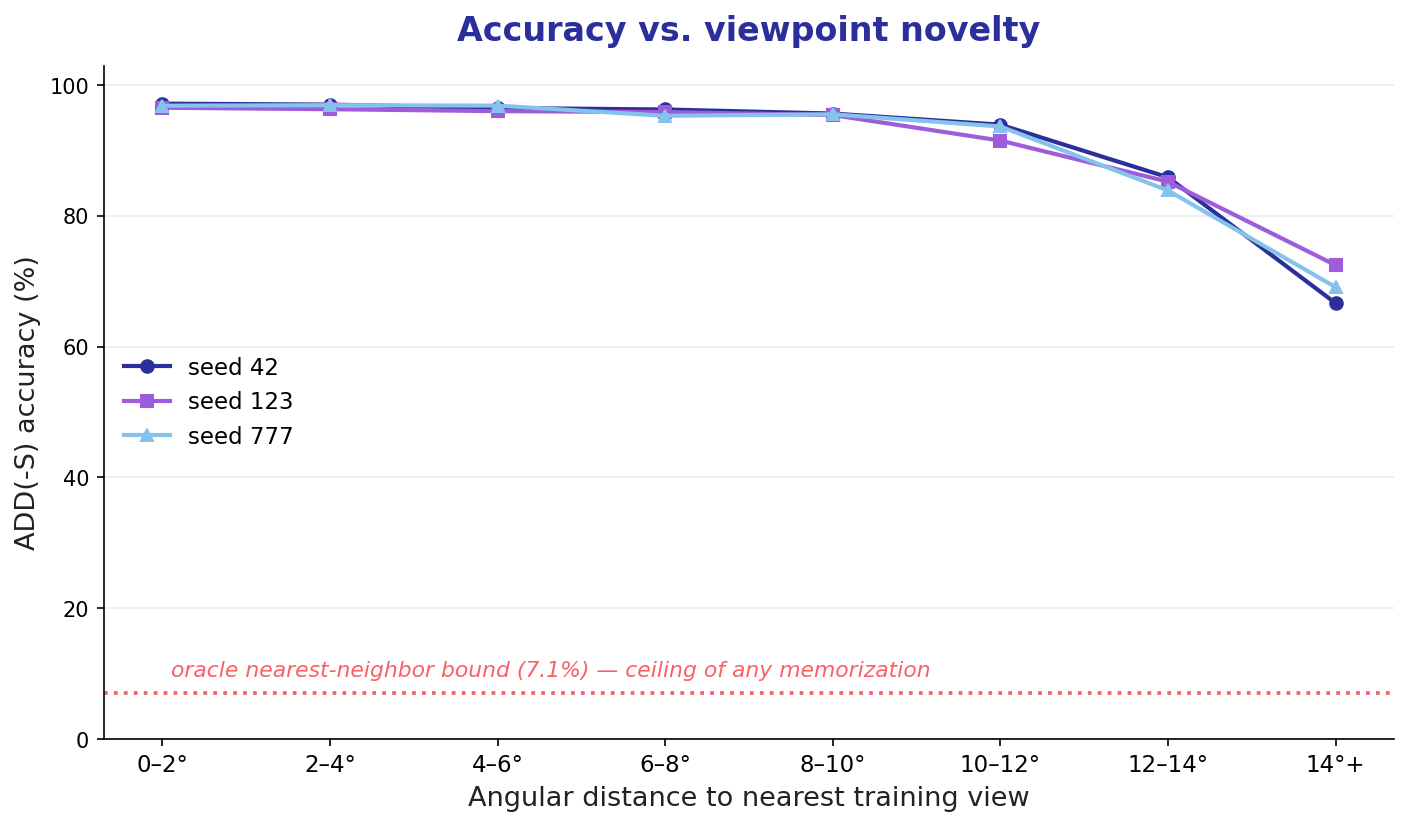
\includegraphics[width=\columnwidth]{figure/v2/gap_curve.png}
    \caption{End-to-end ADD(-S) accuracy as a function of the angular distance between each test view and its nearest training view, for three independent training seeds. The profile is flat up to $12^\circ$ (96.4\% of the test set) and degrades gracefully in the extrapolation tail; the dotted line marks the oracle nearest-neighbor bound, the ceiling of any memorization strategy.}
    \label{fig:gapcurve}
\end{figure}
